\documentclass{report}
\usepackage[utf8]{inputenc}
\usepackage{natbib}
\usepackage{graphicx}
\usepackage[pagestyles]{titlesec}
\usepackage{pdfpages}

\title{Design Document}
\author{AmorosiniCasaliFioravanti}
\date{December 2019}

\titleformat{\chapter}[display]{\normalfont\bfseries}{}{0pt}{\Huge}
\newpagestyle{mystyle}
{\sethead[\thepage][][\chaptertitle]{}{}{\thepage}}
\pagestyle{mystyle}

\begin{document}


\includepdf[pages={1}]{./img/FrontPage}

\chapter{Introduction}
\section{Purpose}
While the RASD presented a general view of the SafeStreets appliction and its features, this document aims to further analyze the system's design and architecture, as well as describing for each of its components their runtime behaviour, integration, interfaces, implementation and testing plans.
This document is mainly intended to be used by the test and development teams as a guidance in the development process, but also to prevent structural degradation during maintainance and extension phases. Nonetheless, the document is also addressed to all the stakeholders who are interested in supervising the development process.

\section{Scope}
SafeStreets: an application that aims to improve the safety of urban areas by giving its users the possibility to report traffic violations to authorities. Users are logged in either as citizen, those who report the violations, and authorities, those who are notified about newly reported violations and are supposed to take action on them.\\
The system is in charge of collecting all the reports, storing them, and notifying the authorities about them. The stored reports are then used to build statistics, find unsafe areas, and compute suggestions on how to improve the safety of such areas. The system may also communicate with local Municipalities' Systems in order to retrieve information about accidents and iussued traffic ticket: in this case some of the above functions are enhanced, and some new functions are enabled (g.e computing statistics on traffic ticked).\\
\newline
Further information about the scope of the application can be found in the Chapter 1 of the RASD.

\section{Definitions, Acronyms and Abbreviations}
\subsection{Definitions}
\begin{itemize}
    \item \textit{Client}: a piece of computer hardware or software that accesses a resource or a service made available by a Server.
    \item \textit{Server}: a device or a computer program that provides resources or functionalities to other programs or devices.
    \item \textit{Firewall}: a network security systems that monitors incoming and outcoming network traffic, applying predefined predefined security rules.
\end{itemize}
\subsection{Acronyms}
\begin{itemize}
    \item \textbf{RASD}: \textit{Requirement Analysis and Specification Document}, the document in which all the requirements and goals of the application are throughly described.
    \item \textbf{API}: \textit{Application Programming Interface}, interface, or communication protocol between Client and Server intendend to simplify the building of the Client-side software.
    \item \textbf{GPS}: \textit{Global Positioning system}, technology widely used to get the user's position.
    \item \textbf{DBMS}: \textit{Data Base Management system}, software that provides organized space memory to store information.
    \item \textbf{OCR}: \textit{Optical Character Recognition}, software dedicated to the detection of characters contained in a document and to their transfer to digital text that can be read by a machine. In this context, OCR will be used to read license plates.
    \item \textbf{UML}: \textit{Unified Modeling Language}, a standard visual modeling language intended to be used for analysis, design, and implementation of software-based systems.
    \item \textbf{MVC}: \textit{Model View Controller}, a software design pattern commonly used to provide user interfaces.
    \end{itemize}
\subsection{Abbreviations}
\begin{itemize}
    \item {[R$_{i}$]}: i-th requirement.
    \end{itemize}
\section{Reference Documents}
\begin{itemize}
    \item Specification document: \textit{SafeStreets Mandatory Project Assignment.pdf}.
    \item Requirement Analysis and Specification Document: \textit{RASD.pdf}.
\end{itemize}
\section{Document Structure}
This document is presented as it follows:
\begin{enumerate}
    \item \textbf{Introduction} presents a general overview, the scope and the purpose of the document.
    \item \textbf{Architectural Design} shows the main components of the system and their relationships. This section will also discuss the architectural choices of the design process.
    \item \textbf{Algorithm Design} presents and discusses the algorithms that will enable the system's functionalities.
    \item \textbf{user Interface Design} provides some further details on the user interface defined in the RASD.
    \item \textbf{Requirement Traceability} maps all the functional requirements defined in the RASD over the components that will accomplish them.
    \item \textbf{Implementation, Integration and Testing Plans} shows the order in which the implementation and the integration of the components will occur, and how the testing phase will be carryed out.
    \item {\textbf{Effort spent}} displays the time spent writing this document by each member of the team.
\end{enumerate}
\chapter{Architectural Design}
\section{Overview}
In this chapter the architectural structure of the system will be discussed at multiple levels of abstraction. A high-level view of the components and their interactions is represented in Figure \ref{fig:overview}. The details will be explained in the following sections.
\begin{figure}[!ht]
	\begin{center}
	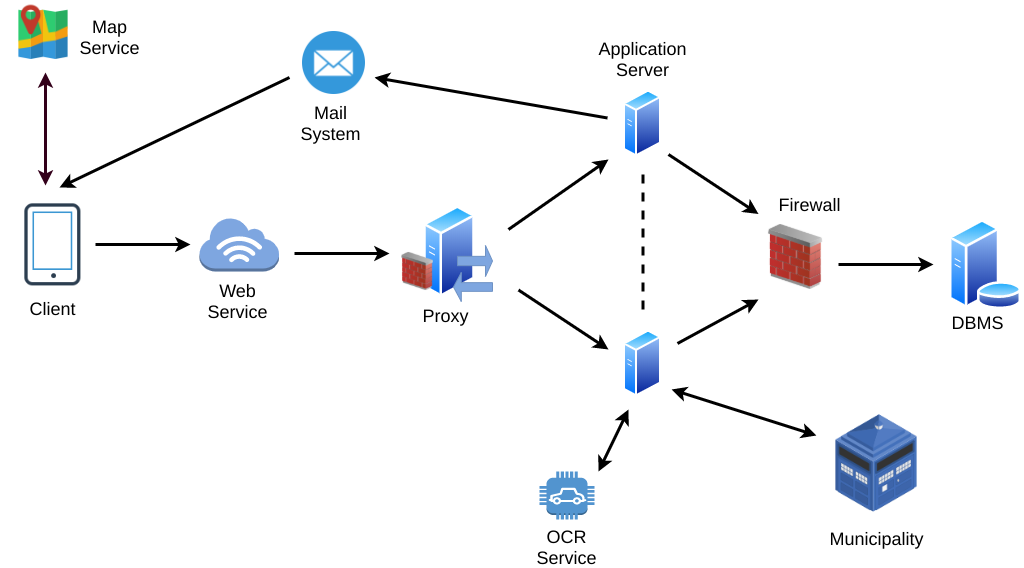
\includegraphics[width=\textwidth]{img/HighLevelOverview.png}
    \end{center}
    \label{fig:overview}
	\caption{High-level overview of the system.}
\end{figure}
\newpage
\section{Component view}
The UML component diagram aims at capturing the internal modular structure of the components, showing how they are connected together in order to form larger components. Components are wired together by using an assembly connector to connect the required interface of one component with the provided interface of another component.
\begin{figure}[!ht]
	\begin{center}
	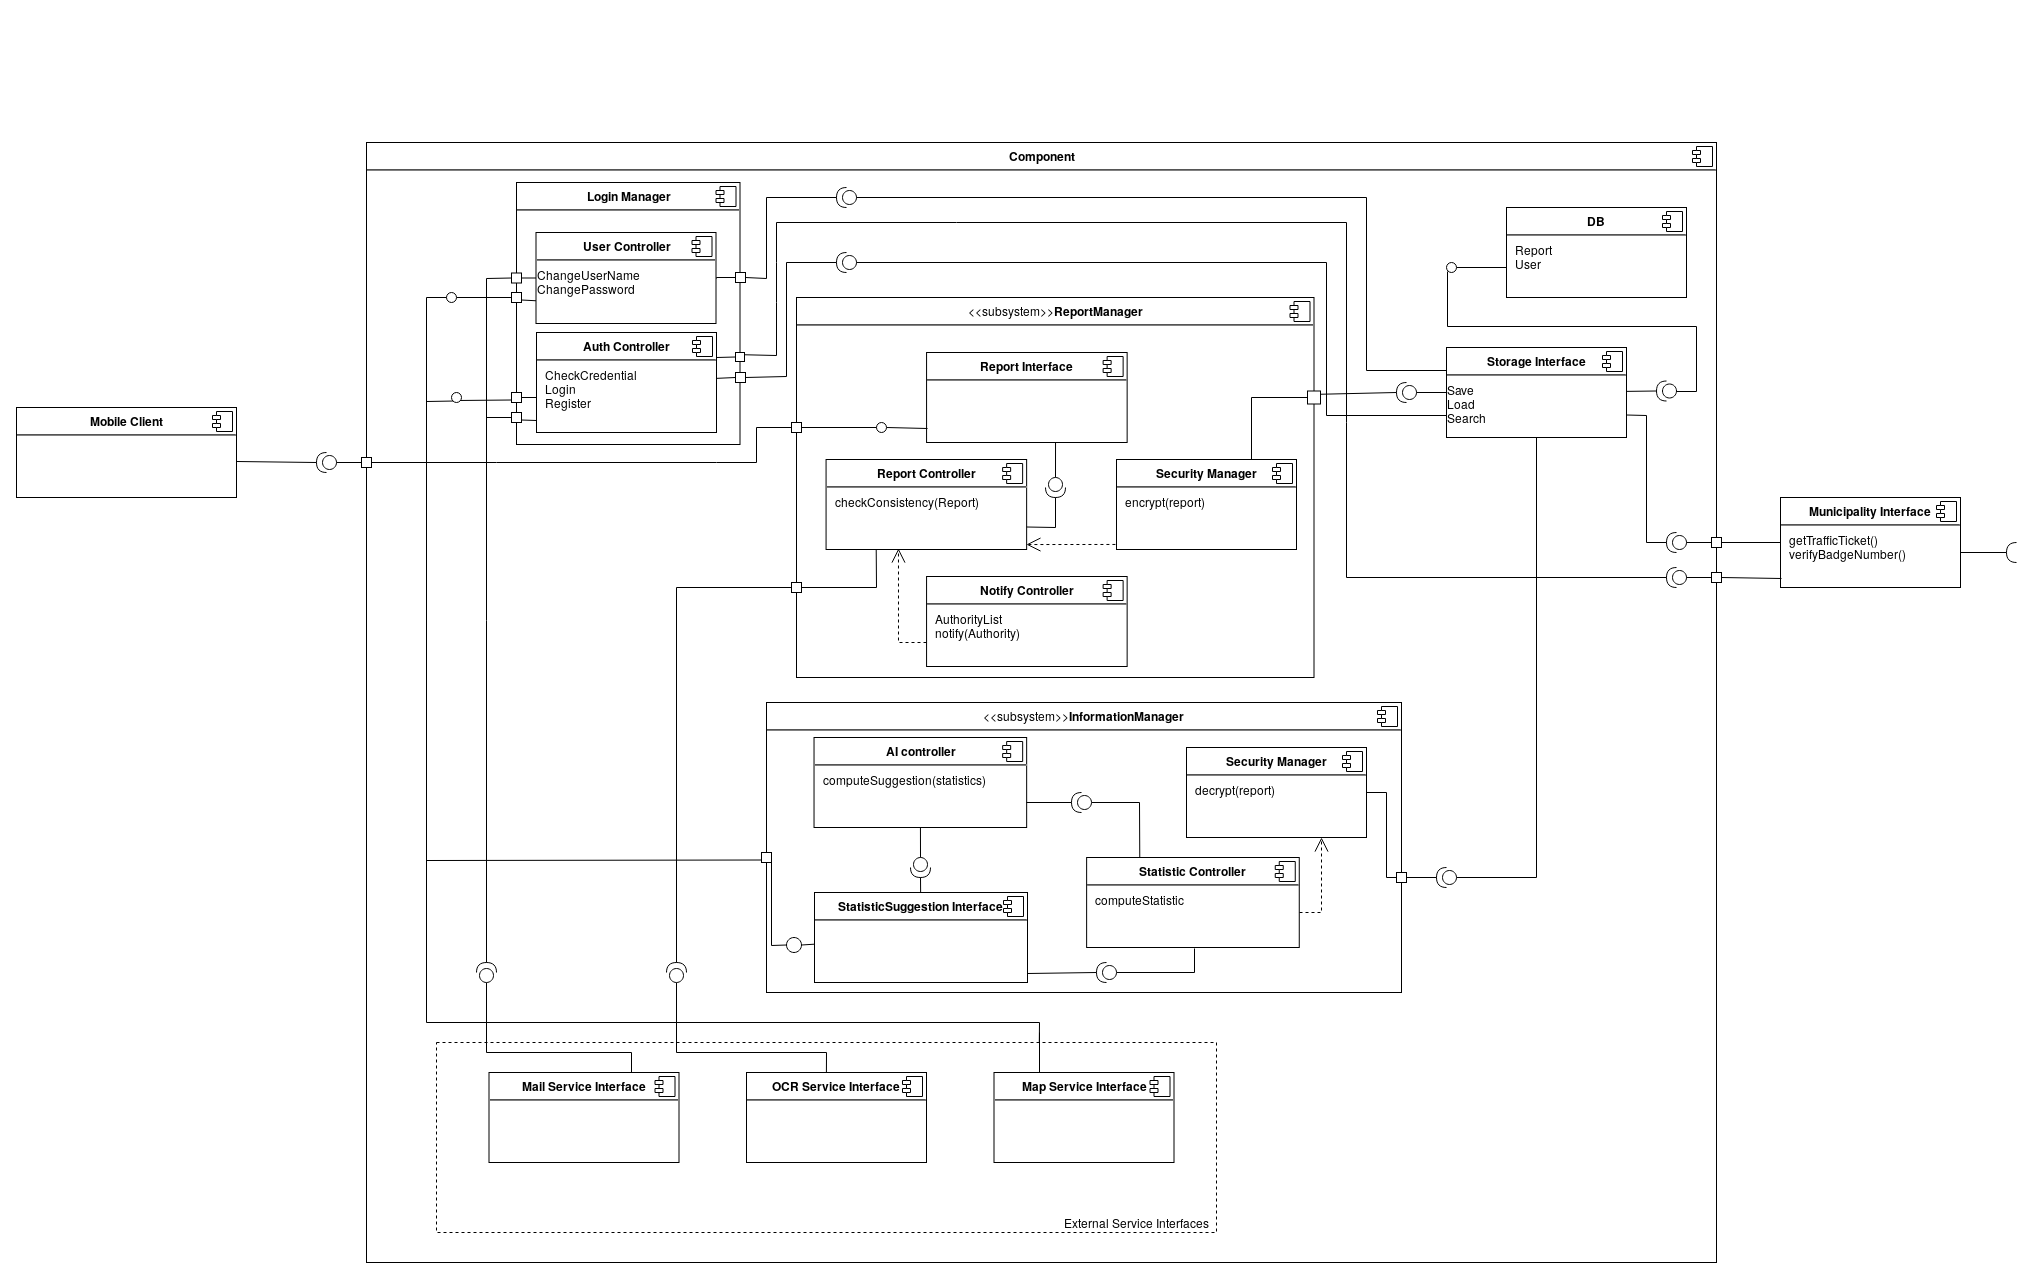
\includegraphics[width=\textwidth]{img/Component2.png}
    \end{center}
    \label{fig:componentdiagram}
	\caption{Component diagram of the system.}
\end{figure}
Below is a description of each component:
\begin{itemize}
\item \textbf{Mobile Client}: the client device that accesses to the functionalities of the entire system. It is implemented as thin client as explained below.
\item \textbf{Login Manager}: it takes care of all the operation related to the registration, login, checking credentials... . It is composed by 2 main components:
\begin{itemize}
    \item \textbf{User Controller}: it takes care of all the operation related to the user's data. It exposes methods to change account credentials and it stores the user's data in the database using the Storage Interface.
\item \textbf{Auth Controller}: it takes care of all the authentication-related operations: it is responsible both for the log in and the registration process, and it also uses the \textit{Storage Interface} to retrieve and store new users' credentials in the databse. During the registration process, the Auth Controller uses the \textit{Mail Service Interface} to communicate with the Mailing Service in order to send registration emails.
\end{itemize}
\item \textbf{Report Manager}: it's a \textit{subsystem} component in charge of all the processing functions on the newly recieved reports:
\begin{itemize}
    \item \textbf{Report Interface}: it exposes to the User an interface in the form of a blank report to be compiled.
    \item \textbf{Report Controller}: it aims to check the validity of the sent reports. To do this, it communicates with the Report Interface to check them as soon as they are recieved.
    \item \textbf{Notify Controller}: the role of this component is to select the correct authorities to notify based on their municipality, using his \textit{AuthorityList}. It depends on the Report Controller, in the sense that it will notify the authorities only if the check of the report is successful and the type of the report is \textit{Traffic Violation}.
    \item \textbf{Security Manager}: it takes care of the security side: as specified in the Security section of the RASD, before being stored, the report is encrypted and then stored in the database. This task is accomplished by this specific component, that also depends on the Report Controller due to the fact that if the report doesn't pass the check verification, it will be discarded and therefore never encrypted.
\end{itemize}
\item \textbf{Storage Interface}: its main purpose is to retrive the reports from the database, decopuling the other components of the system from the particular data sources. This component is also in charge of authenticating the system with local municipalities' systems, and eventually crossing their data with SafeStreets' own information.
\item \textbf{DB}: this component represent the DBMS, which provides an interface to read and store data. Both user credentials and submitted reports are stored in the database.
%\item \textbf{Notification Interface}: it's goal is to send push notifications to all the authorities identified by the \textit{Notification Controller}.
\item \textbf{Information Manager}: a \textit{subsystem} in charge of building statistics, compute safety suggestions and deploy them to the users who requested them.
    \begin{itemize}
        \item \textbf{StatisticsSuggestions Interface}: it exposes to the users the latest statistics and safety suggestions. As aready mentioned in the RASD, the exposed data may be different according to the level of visibility granted to different users.
        \item \textbf{Statistics Controller}: it analyzes the stored reports to build statistics and find unsafe urban areas. Depending on the agreements with local municipalities, this component can also compute statistics on iussued traffic tickets or refine its statistics about accidents.
        \item \textbf{AI Controller}: its role is to analye previously built statistics and compute safety suggestions. These suggestions are addressed to the authorities who use the SafeStreets application.
        \item \textbf{Security Manager}: similarly to the one described in the Report Manager subsystem, this component is in charge of decrypting stored reports so that they can be analyzed. To ensure that no report is ever altered, this component can perform read-only operations, whereas the one in the Report Manager is the ony one which disposes of write permissions.
    \end{itemize}
\item \textbf{Municipality Interface}: it is a component external respect to the system. It deals with interfacing with the Authentication Control to confirm the validity of the badge number of the authorities and it is useful to retrieve data relative to the traffic tickets, in this case only if the Municipality gives the permission to treat this data.
\item \textbf{External Services Interfaces}: it's a set of components whose main task is to make an API call to the corresponding third party service.
    \begin{itemize}
        \item \textbf{Mail service Interface}: it's an interface towards the mailing service, which is in charge of sending confirmation mails at the end of the registration process.
        \item \textbf{OCR service Interface}: it calls a service used by the Report Manager to read license plates from pictures submitted in the reports by users.
        \item \textbf{Map service Interface}: it provides the users with the functionality of visualizing the statistics (and their own position) on a geographic area using an interactive map.
\end{itemize} 
\end{itemize}
\section{Deployment view}
In this section it is described the deployment view of the components inside the system. The deployment diagram shows the distribution of components of the hardware.
\begin{figure}[!ht]
	\begin{center}
	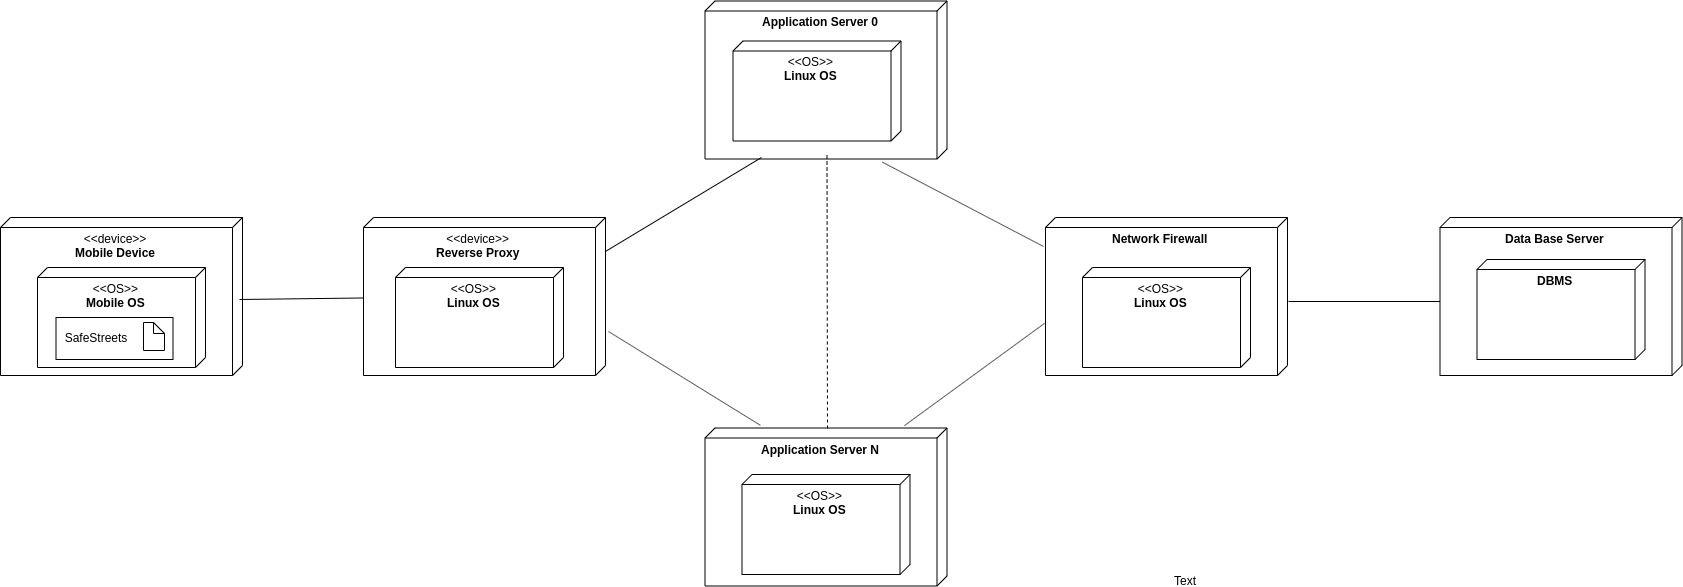
\includegraphics[width=\textwidth]{img/DeploymentView.png}
    \end{center}
    \label{fig:deploymentview}
	\caption{Deployment diagram of the system.}
\end{figure}\\
The system is composed of a multitier architecture and each specific role is clarified below.\\
\begin{itemize}
    \item \textbf{Client}\\
    The first tier contains the client mobile machines which have installed SafeStreets application
    to access all its functionalities.\\
    \item \textbf{Reverse Proxy}\\
    The second tier contains a reverse proxy to implement load balancing on the several requests to access the application servers.
    Furthermore, it is a cacheble component who can speed-up the most frequent requests.
    Linux machine have been chosen for safety and simplicity. \\
    \item \textbf{Application servers}\\
    This is the middleware level of the application where all the computations happen. The servers
    are distributed to increase the scalability of the network, they are also part of the second tier.\\
    \item \textbf{Firewall}\\
    The access to the Database is protected from a firewall to avoid unauthorized accesses to sensible data.\\
    \item \textbf{Database Server}\\
    This is the last layer of the architecture. All the data are stored here structured in a relational DBMS.
\end{itemize}
\newpage
\section{Runtime view}

\subsection{Registration Runtime View}
\begin{figure}[!ht]
	\begin{center}
	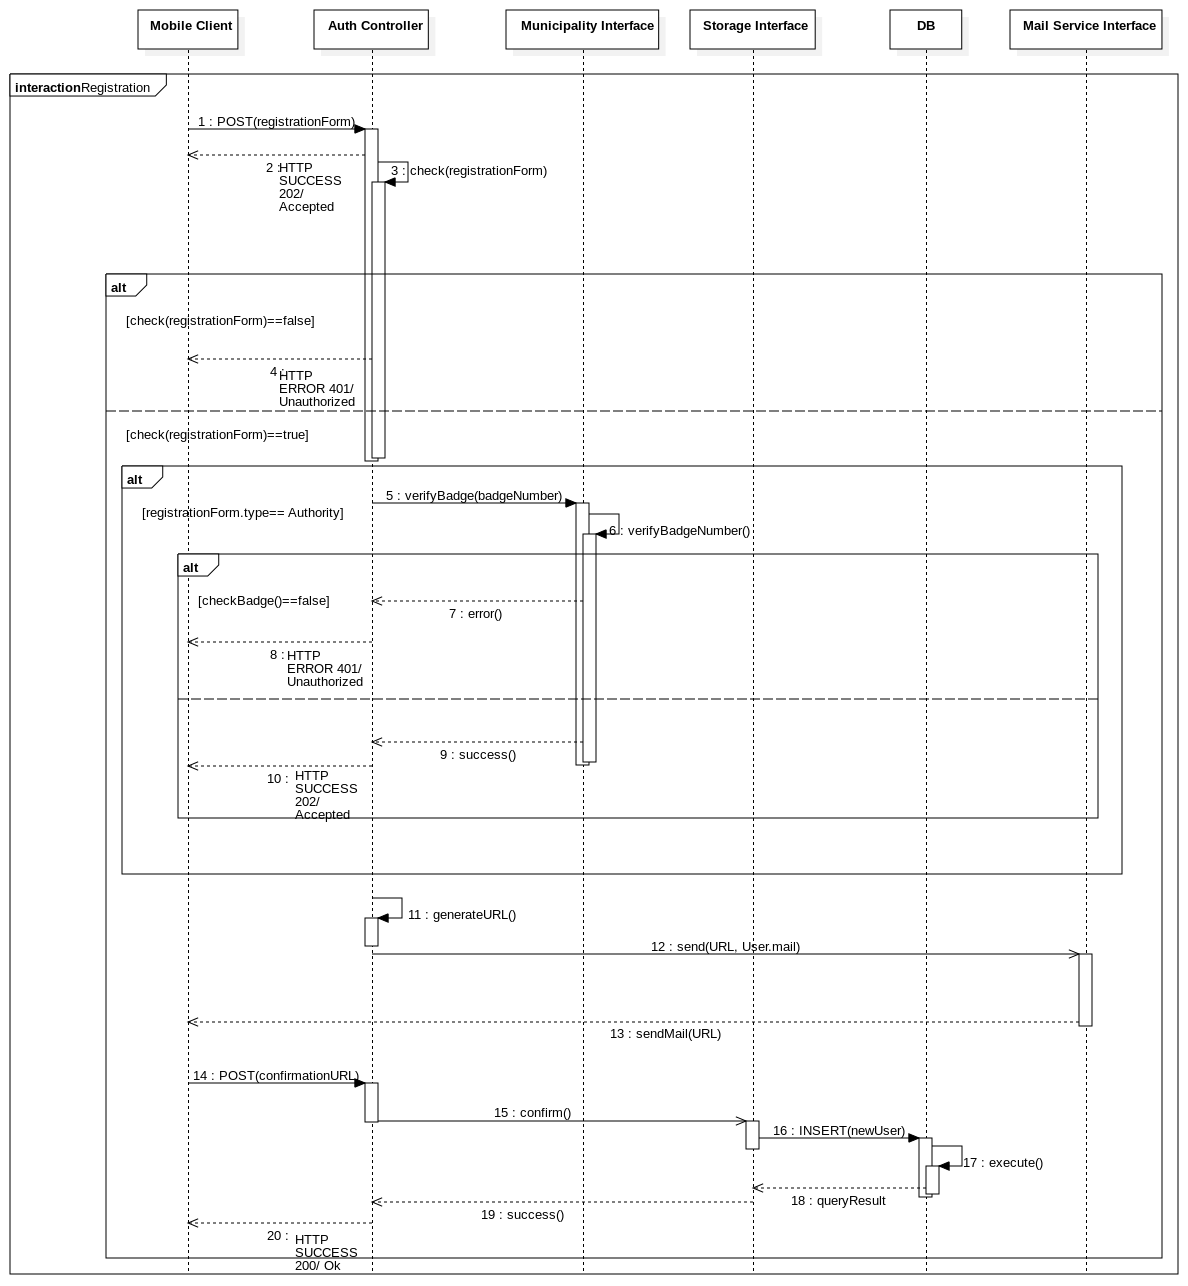
\includegraphics[width=\textwidth]{img/Registration.png}
    \end{center}
    \label{fig:RegistrationSD}
	\caption{Registration Runtime View.}
\end{figure}
The Guest has to register before accessing the functionalities of the application. The Guest fills a form containing the necessary information. The information are sent to the Application Server through an HTTP POST. The \textit{Authentication Controller} handles the request, verifies if the information are correct and complete. Then it generates an URL, that it is forwarded by the external mailing system to the Guest. Once the Guest confirms the registration clicking on the URL link, the \textit{Storage Interface} insert the new User with its credentials in the Database, so from this moment on the new User is able to authenticate and to use the functionalities of the application.
In the event that is an Authority to register, once the Authority has filled and sent the form, the \textit{Authentication Manager} contacts the \textit{Municipality Interface} to be sure that the entered badge number is correct. If the Municipality Interface replies that the provided badge number is correct, the registering procedure is the same as before; otherwise an HTTP Error is send back to the Guest that has sent the information.    
%\newpage
\subsection{Login Runtime View}
\begin{figure}[!ht]
	\begin{center}
	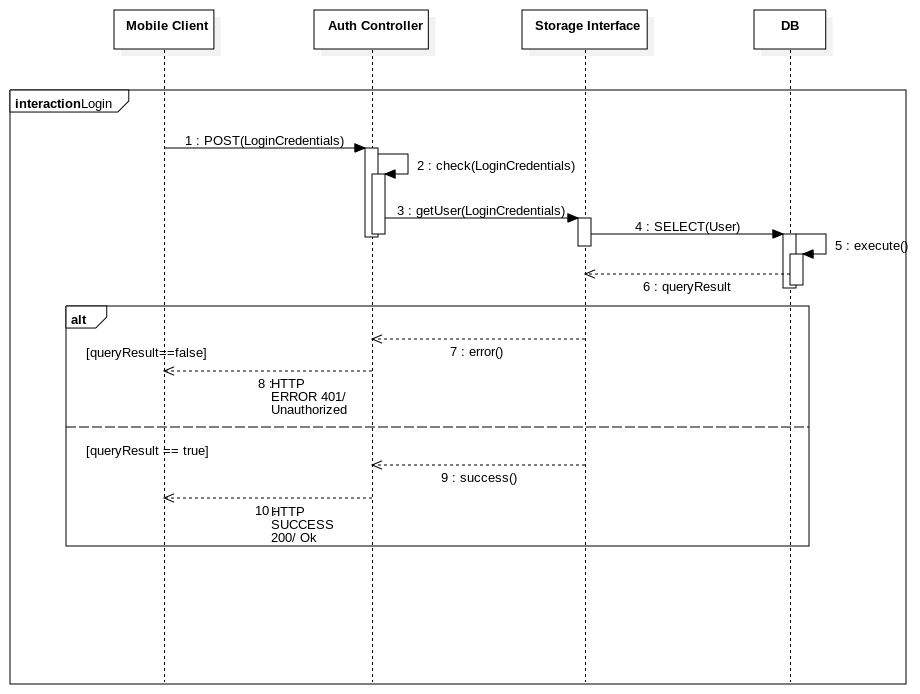
\includegraphics[width=\textwidth]{img/Login.png}
    \end{center}
    \label{fig:LoginSD}
	\caption{Login Runtime View.}
\end{figure}
The Client to access the functionalities of the application has to log in (clearly as specified before he/she must be registered). The Client fill the Log in form with his/her credentials. The provided information are sent to the Application Server through an HTTP POST. The \textit{Authentication Controller} handles the request and checks the information. It interfaces with the \textit{Storage Interface} that runs a SELECT query on the Database to verify the existence of the User. If the query return a result an HTTP Success message is return to the Client that now is able to access to the functionalities of the application, otherwise an HTTP Error is send back to the Client that is not able to log in successfully.
%\newpage
\subsection{Send Report Runtime View}
\begin{figure}[!ht]
	\begin{center}
	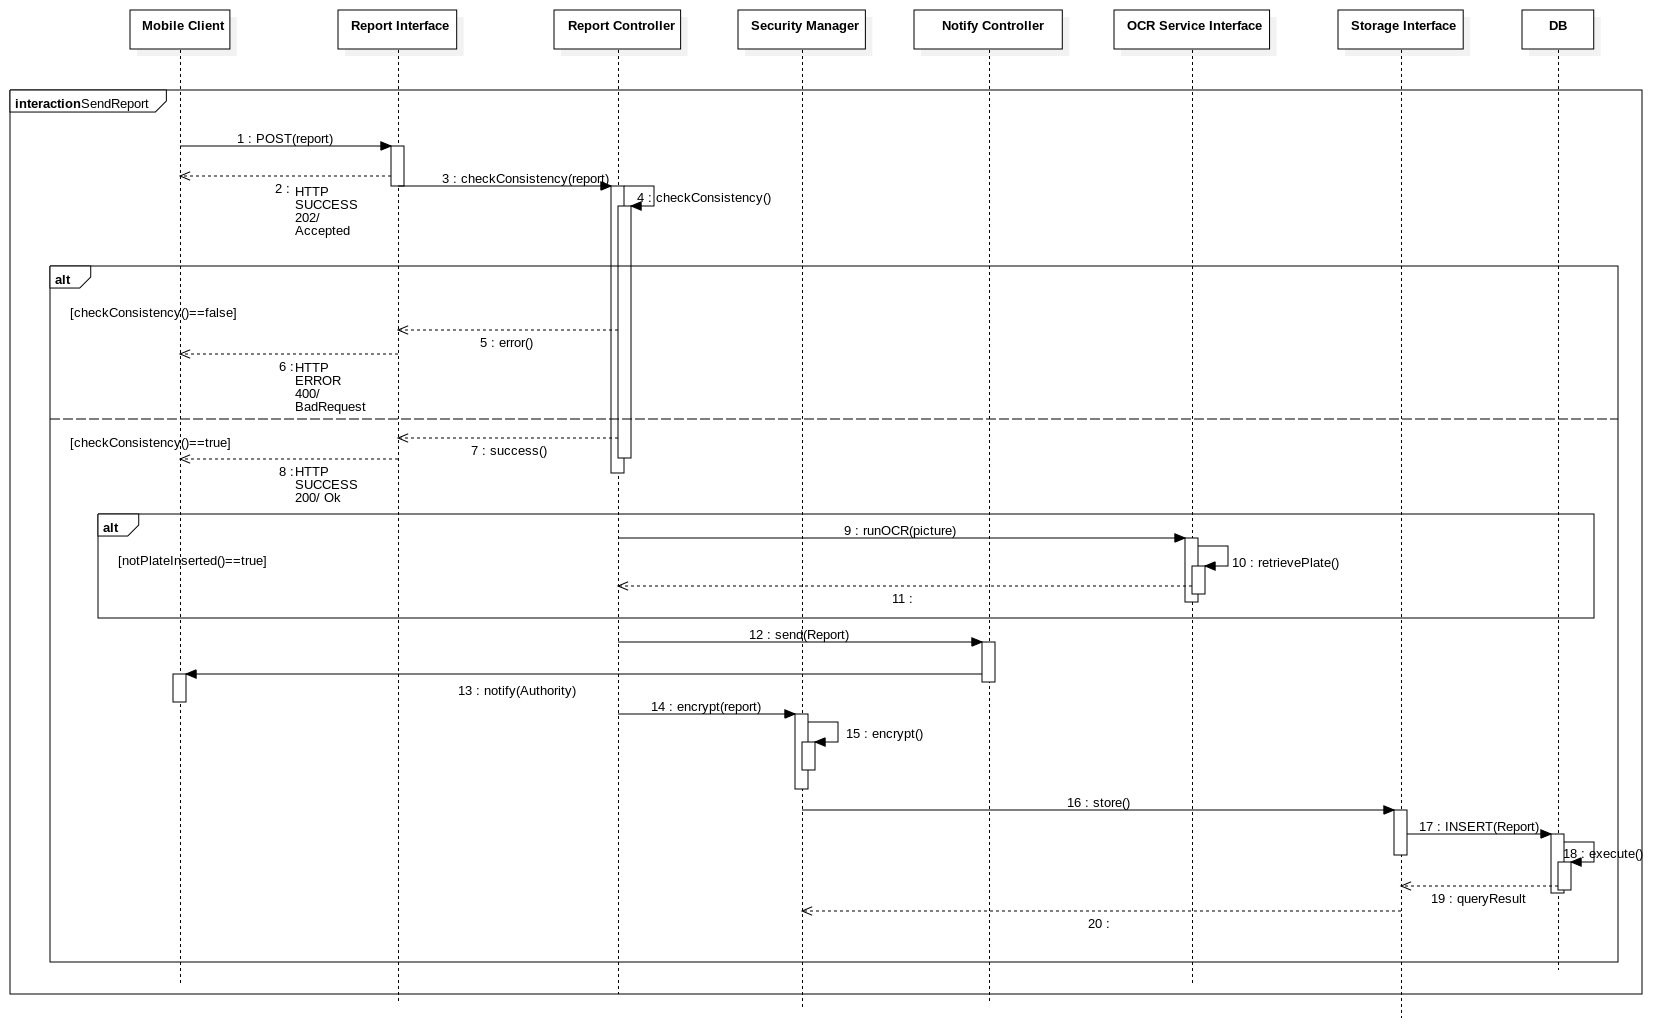
\includegraphics[width=\textwidth]{img/SendReport.png}
    \end{center}
    \label{fig:SendReportSD}
	\caption{Send Report Runtime View.}
\end{figure}
The User (Citizen in this case) is logged in and opens the section to send the report. The \textit{Report Interface} provides the report form that has to be filled. The \textit{Report Interface} interfaces also with the \textit{Report Controller}, so once the report is compiled and sent by the User, the Report Interface shows it to the Report Controller so that it can checks its consistency. 
If the User has not inserted the license plate in the report, the Report Controller uses an external OCR service system, that execute an OCR algorithm to retrieve the license plate from the picture provided by the User.
At this point, when all the information are avaiable, the report is shared with the \textit{Notify Controller} which will check its Authority list to notify the right Authority.
Then using the \textit{Security Manager} the report is encrypted and stored in the Database using the \textit{Storage Interface}, that runs an INSERT query. 
\newpage
\subsection{Compute Statistics Runtime View}
\begin{figure}[!ht]
	\begin{center}
	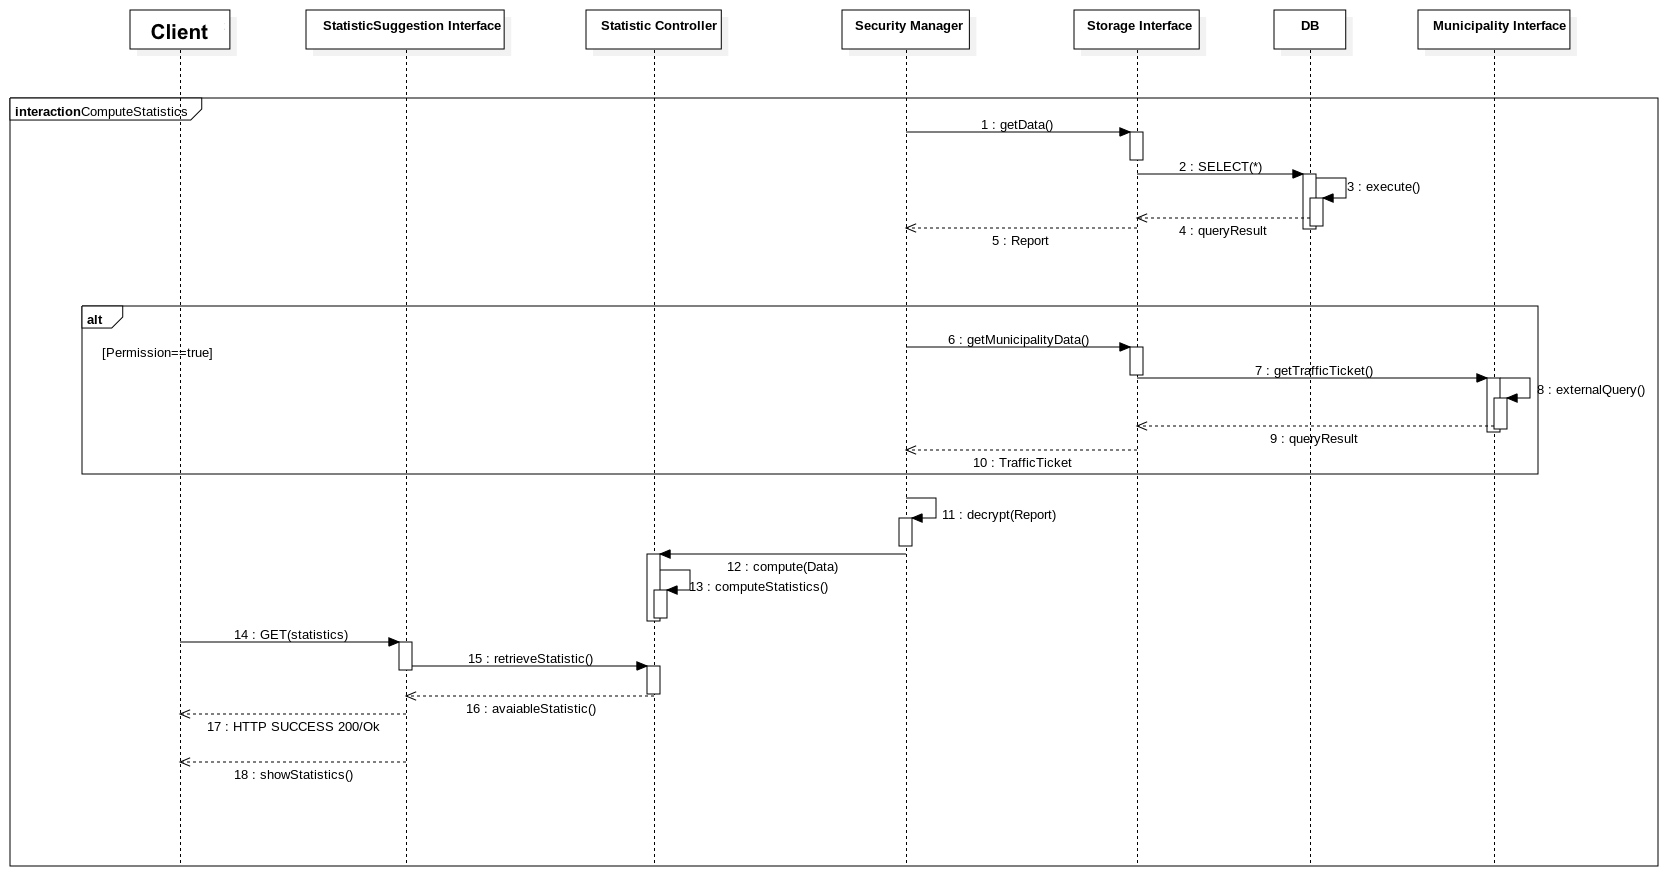
\includegraphics[width=\textwidth]{img/ComputeStatistics.png}
    \end{center}
    \label{fig:ComputeStatisticSD}
	\caption{Compute Statistics Runtime View.}
\end{figure}
The procedure to compute the statistics and the suggestions is performed by the \textit{Information Manager}. In particular the \textit{
Security Manager} uses the Storage Interface to retrieve all the report. So it decrypt them and requests the \textit{Statistic Controller} to compute the statistics on them. If the Municipality has given the permission to process the data relative to the traffic tickets, the Storage Interface retrieve them contacting the \textit{Municipality Interface} (external to the system). As soon as the statistics are available, the Statistic Controller provides them to the StatisticsSuggestions Interface and moreover provides them to the \textit{AI Controller} that runs some algorithm to compute useful suggestions based on the avaiable statistics.
When avaiable, the suggestions, as the statistics, are provided to the StatisticsSuggestions Interface. So when an User goes in to the Statistics section, the StatisticsSuggestions Interface shows him everything. 
In particular if the User is an Authority, suggestions are also shown.  


\section{Component interfaces}
\subsection{API REST}
\begin{center}\large{\textbf{Authentication Controller}}\end{center}
The \textit{Authentication Controller} provides methods for login and registration.
This Controller also makes the check on the authority credential calling the methods inside \textit{Municipality Interface}.
The Authentication Controller exposes the following methods: \\

\begin{center}{\textbf{Registration}}\end{center}
\begin{tabular}{| l | p{8cm} |}
    \hline
    \textbf{Endpoint} & */auth/register \\
    \hline
    \textbf{Method} & POST \\
    \hline
    \textbf{Data Params} & username: [string] \newline email: [string] \newline password: [string] \newline If the user is an authority: \newline municipality: [string]\\
    \hline
    \textbf{Success Response} & code: 200 \newline content: {message: "Registration successful"}\\
    \hline
    \textbf{Error Response} & \newline code: 422 UNPROCESSABLE ENTRY \newline body: {error: "Registration data not correct"} \newline\newline code: 401 \newline body: {"error": "Provided email does not exist"}   \\
    \hline
    \textbf{Notes} & Allows the user to request the registration as citizen or authority. \\
    \hline
\end{tabular}
%%%%%%%%%%%%%%%%%%%%%%%%%%%%%%

\begin{center}{\textbf{Login}}\end{center}
\begin{tabular}{| l | p{8cm} |}
	\hline
	\textbf{Endpoint} & */auth/login \\
	\hline
	\textbf{Method} & POST \\
	\hline
	\textbf{Data Params} & username: [string] \newline password: [string]\\
	\hline
	\textbf{Success Response} & code: 200 \newline content: {accessToken: [string]}\\
	\hline
	\textbf{Error Response} & \newline code: 422 UNPROCESSABLE ENTRY \newline body: {error: "Login data not correct"} \newline \newline code: 401 UNAUTHORIZED \newline body: {error: "wrong Username or Password"} \\
	\hline
	\textbf{Notes} & Allows the client to obtain an authentication Token \\
	\hline
\end{tabular}
%%%%%%%%%%%%%%%%%%%%%%%%%%%%%%

\begin{center}{\textbf{Activate Account}}\end{center}
    \begin{tabular}{| l | p{8cm} |}
        \hline
        \textbf{Endpoint} & */auth/activate \\
        \hline
        \textbf{Method} & GET \\
        \hline
        \textbf{Data Params} & \\
        \hline
        \textbf{Success Response} & code: 200 \newline content: {message: "Account activated"}\\
        \hline
        \textbf{Error Response} & code: 404 NOT FOUND \newline content: {error: "Incorrect activation code"} \newline \newline code: 401 \newline body: {"error": "Account not activated"} \newline \newline code: 401 \newline body: {error: "Wrong password"} \ \newline code: 401 \newline body: {error: "Provided email does not exist"}   \\
        \hline
        \textbf{Notes} & Allows a Client to activate the account \\
        \hline
    \end{tabular}
%%%%%%%%%%%%%%%%%%%%%%%%%%%%%%%%%%
%%%%%%%%%%%%%%%%%%%%%%%%%%%%%%%%%%
\begin{center}\large{\textbf{Report Controller}}\end{center}
    The \textit{Report Controller} provides methods to check and send consistet reports to the \textit{Notify Controller}.
    The Authentication Controller exposes the following methods: 

\begin{center}{\textbf{Send Report}}\end{center}
    \begin{tabular}{| l | p{8cm} |}
        \hline
        \textbf{Endpoint} & */send \\
        \hline
        \textbf{Method} & POST \\
        \hline
        \textbf{Data Params} & data: [string] \newline time: [string] \newline license plate: [string] \newline picture: [png/jpg]\\
        \hline
        \textbf{Success Response} & code: 200 \newline content: {message: "Registration successful"}\\
        \hline
        \textbf{Error Response} & \newline code: 400 BAD REQUEST \newline body: {error: "Data not correct"}\\
        \hline
        \textbf{Notes} & Allows the user to request the registration as citizen or authority. \\
        \hline
    \end{tabular}
%%%%%%%%%%%%%%%%%%%%%%%%%%

\begin{center}{\textbf{Send Report}}\end{center}
    \begin{tabular}{| l | p{8cm} |}
        \hline
        \textbf{Endpoint} & */send \\
        \hline
        \textbf{Method} & POST \\
        \hline
        \textbf{Data Params} & data: [string] \newline time: [string] \newline license plate: [string] \newline picture: [png/jpg]\\
        \hline
        \textbf{Success Response} & code: 200 \newline content: {message: "Registration successful"}\\
        \hline
        \textbf{Error Response} & \newline code: 400 BAD REQUEST \newline body: {error: "Data not correct"}\\
        \hline
        \textbf{Notes} & Allows the user to request the registration as citizen or authority. \\
        \hline
    \end{tabular}
%%%%%%%%%%%%%%%%%%%%%%%%%%


\section{Selected architectural	styles and patterns}
The following architectural patterns are used to build the structure of the system in order to provide all the services of SafeStreets application.\\

\begin{center}\large{\textbf{Client-Server Architecture}}\end{center}
Client-Server architecture is a computing model that features two roles: a Server that hosts, delivers and manages most of the resources and services, and a Client which exploits them.
\begin{center}\large{\textit{Motivations}}\end{center}
\noindent This structure provides several advantages:
\begin{itemize}
    \item Scalability and Mantainability: it is possible to repair or add more resources to the architecture without significative service interruptions.
    \item Security: the server is able to manage what levels of access each user can have with respect to specific resources.
\end{itemize}\vspace{2mm}

\begin{center}\large{\textbf{Three-tiered Architecture}}\end{center}
This type of architecture is a kind of Client-Server paradigm where three tiers are phisically separated:
\begin{itemize}
	\item The \textit{presentation tier} is the top-most level of the architecture, which provides an interface that users can use to directly access the application. 
	It is the top-most tier and the only one accessible from the Client.
	\item The \textit{application tier} runs the business logic of the application and executes functions that elaborate data. 
	A Reverse Proxy is needed to handle the Client requests and to balance the workload, the requests are forwarded to 
	the application serves in order to provide the right data.
	\item The \textit{database tier} includes the data persistence mechanisms and the data access layer that encapsulates 
	the persistence mechanisms and exposes the data.
\end{itemize}
\begin{center}\large{\textit{Motivations}}\end{center}
A multi-tier application architecture provides a model with several advantages: in this way developers can create flexible and reusable 
applications that can be modified, enhanced or maintained just by operating on a specific layer, instead of reworking the entire application. Furthermore, a general multitier architecture can also help improve the development efficiency by allowing teams to focus on their core competencies.

\begin{figure}[!ht]
	\begin{center}
	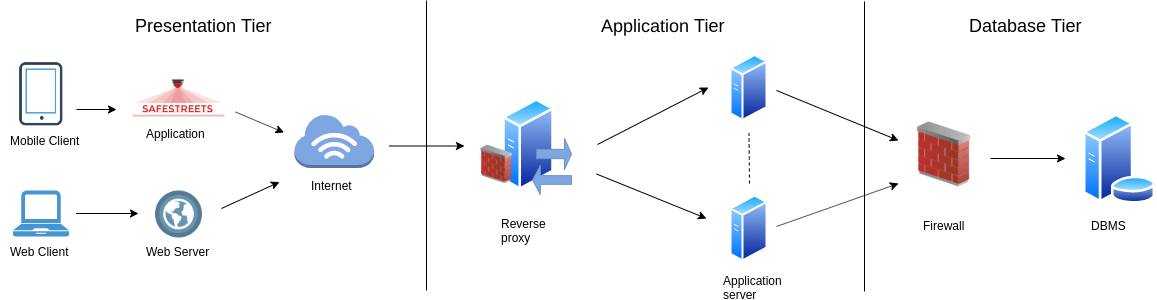
\includegraphics[width=\textwidth]{img/TiersArchitecture.png}
	\end{center}
	\caption{Three-tier architecture schema.}
\end{figure}

\begin{center}\large{\textbf{Thin Client}}\end{center}
A thin Client is a lightweight computer which does most of the computation in a remote Server. In this paradigm in fact, since the Servers take care of several duties such as storage 
of data and performing calculations, the Client does not need to have a large memory or powerful computing capabilities to run the application.
\begin{center}\large{\textit{Motivations}}\end{center} 
The application is thought mostly for mobile phones which do not have great computing power or very large memories. Thanks to a thin client a internet connection is virtually the only requirements to use the application. Furthermore, this architecture simplify the front-end implementation by shifting most of the execution to the servers.

\begin{center}\large{\textbf{MVC Design Pattern}}\end{center}
Model-View-Controller is a software design pattern commonly used to develop user interfaces. Indeed, this pattern is used for the front-end implementation of the application. It divides the program logic in three interconnected elements: \textit{model} that directly manages data and rules of the application, \textit{view} which handles any representation of data, \textit{controller} that 
accepts input and converts it to commands for the model or view. This mechanism is used to separate internal representation of information from the ways information is presented to and accepted from the user. \\
\begin{center}\large{\textit{Motivations}}\end{center} 
MVC allows full encapsulation of objects. This means that each component can be changed without creating issues to other components.
Furthermore, MVC provides decopuling of its components, which means that developers are able to work in parallel on different components of the pattern without interfering with each other.

\begin{center}\large{\textbf{Reverse Proxy Design Pattern}}\end{center}
A simple proxy acts as an interface to refer an object in another machine. The reverse proxy offers a single point of access (with HTTP) to multiple Clients who want to access to several application servers. In practice, it is a wrapper for an object behind the scenes. 
Proxies also provides extra functionalities such as data caching (g.e. store the newest statistics available) and security (g.e. client-side firewall).\\
\begin{center}\large{\textit{Motivations}}\end{center} 
It is useful to organize the requests of multiple clients and to save frequent requested informations. It also protects the application servers from external attack and slightly improve the overall performances.

\section{Other Architecture}
\begin{center}\large{\textbf{REpresentational State Transfer}}\end{center}
REST is an architectural software type that has become a standard in the creation of Web API. REST describes all type of interfaces capable of exchange data through HTTP, without using auxiliary technologies like cookies or other protocols. This architecture make the communication client-server totally stateless (every request is independent from the others).\\ An HTTP method show the operation to do for accessing an URL. The requests are written in JSON code.
\begin{center}\large{\textit{Motivations}}\end{center}
We decide to use REST to simplify the design and the implementation of the application. Indeed, the developers do not need to take in account the traceability of states.


\end{document}